%\addcontentsline{toc}{chapter}{Development Process}
\chapter{Experiment Methods}

\section{Overview}

The technical outcome of this project was to produce an image analysis pipeline. Broadly speaking the pipeline can be broken into four distinct components. These are feature detection and extraction, dimensionality reduction, quality evaluation, and visualisation components. This section discusses the how the chosen techniques where implemented. 

\section{Techniques}

\subsection{Preprocessing}
Very little preprocessing of the images has been used in this project. Each of the mammograms (real and synthetic) has an accompanying binary mask which is used to remove the background and pectoral muscle (see section \ref{sec:datasets}). The skin around the edge of the breast can cause issues with the blob and line detection due to the intense response during image acquisition. As we are only interested in structure within the parenchyma binary morphological erosion was performed on the breast masks using a disk shaped kernel with a radius of 30 pixels to remove the edge of the breast, preserving only the parenchyma.

\subsection{Features}
\label{sec:experiment-features}
In this project we have used four different types of image features to build a feature space from the mammogram datasets. We have used two different types of shape features. One to detect blobs and one to detect linear structure. Both of these features intrinsically define a ROI within the mammogram. From the ROIs defined by these features we can extract intensity features (based on the image histogram of the ROI) and texture features (in the case of this project use the GLCM of the patch).

\subsubsection{Blob Features}
\label{subsubsec:implementation-blob-features}
The blob detection was achieved by following an approach similar to that described by Chen et al. \cite{chen2013multiscale, chen2013mammographic}. This is a multi-scale approach based on building a Laplacian of Gaussian (LoG) pyramid over ten different scales.

A LoG pyramid is created by convolving an image with a two dimensional kernel that is the combination of a Gaussian kernel with the Laplace operator over a variety of different scales. The response from filter will show sharp peaks anywhere there is a sharp change of intensity. Performing this operation over multiple scales given the resulting response different levels of granularity relative to the width of the Gaussian used.

To obtain a multi-scale view but retain comparative performance (due to the very large size of mammographic images) instead of increasing the size of the kernel the sigma of the Gaussian is fixed to 8.0 and the image is smoothed and downscaled by a factor or $\sqrt{2}$ instead. Once the image has been convolved with the LoG kernel, the resulting image is upscaled to full size. Finally a peak peak detection algorithm is run to find the all maxima within resulting filtered image.

Each of the mammographic images in the real dataset come with a set of breast masks which segment the tissue of the breast from the result of the image (such as the pectoral muscle). This helps to ensure that we are detecting the only within the parenchyma but causes issues due to a large edge response produced from the LoG kernel around the edge of the breast. In Chen's thesis this effect was dealt with by means of a ``deformable" convolution. The image is convolved with a standard image kernel when the area of the kernel is entirely within the mask area. When the kernel being convolved falls outside of the mask the filter kernel is modified so that it returns zero outside of the mask and the LoG response normalised by the number of nonzero pixels otherwise.

For each scale image produced the local maxima are detected using maximum filter and a conservative threshold. The resulting position of the peak defines the location of the blob detected in the image while the effective sigma of the Gaussian for the scale of the image $\sigma k i$ (where $i$ is the scale and $k$ is the downscale factor equal to $\sqrt{2}$) is the radius of the blob.

\begin{figure}[H]
	\label{fig:blob-detection}
	\centering
	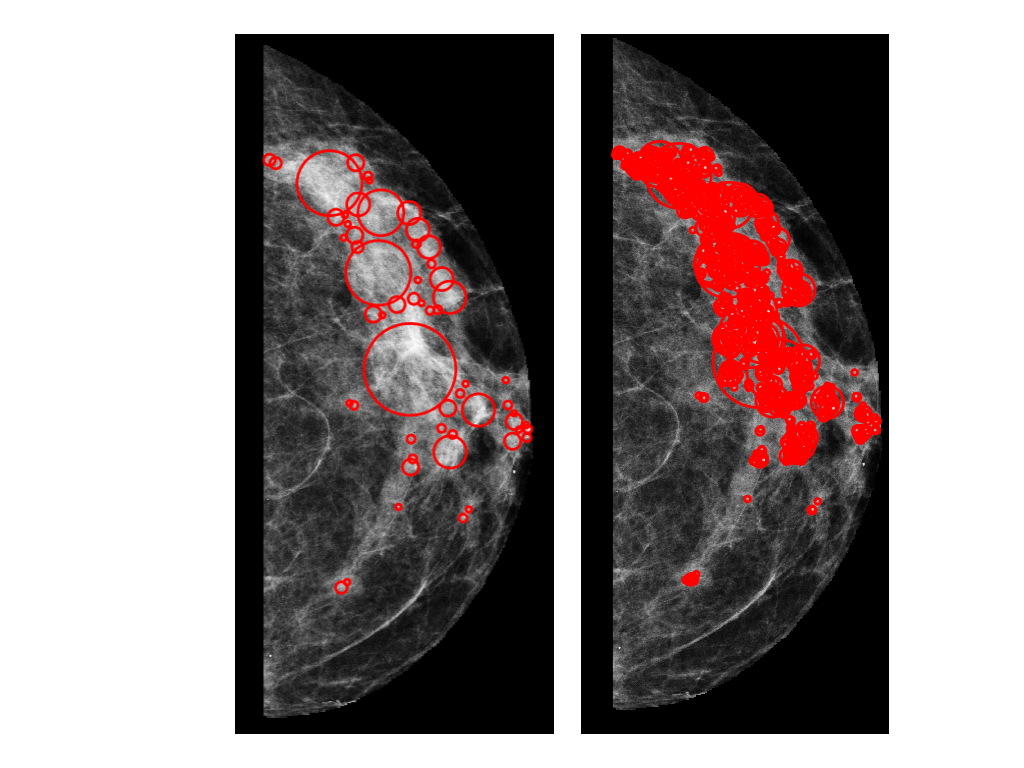
\includegraphics[width=0.8\textwidth]{Images/blob-detections.png}	
	\caption{Example image showing the raw detections (left) and the results of merging the blobs (right).}
\end{figure}

This procedure returns a very large number of responses with many overlapping detections. Since we are only interested in the blob that best characterises the size of the detected peak, a blob merging and pruning strategy is employed to remove redundant blobs. As we are only concerned with blobs that characterise patterns within the parenchyma all blobs whose radius falls outside of the bounds of the image mask are removed. 

Next a thresholding technique is used to remove blobs that fall below a certain level of intensity. The area of the image covered by the blob is categorised into 9 clusters. The average intensity of each cluster is computed and the top 5 clusters are selected. The threshold used is defined to be the average intensity of the top five most intense clusters across all blobs less the standard deviation of those same clusters. 

In Chen's thesis the clustering is performed using the Fuzzy c-means algorithm while in my implementation I have used the k-means algorithm. The result of this is that the algorithm requires more clusters (5 compared to only the top 3 clusters in Chen's thesis) to achieve comparable results.

After these operations the number of blobs detected is significantly reduced but there are still a large number of blobs which significantly overlap one another in high density regions. To achieve a better representation of the distribution of high density tissue in the mammogram, blobs are merged according to how they interact one another. The intersections are classified into one of three categories:

\begin{itemize}
	\item External: $d \geq r_A + r_B$
	\item Intersection: $r_A - r_B < d < r_A + r_B$
	\item Internal: $d \leq r_A + r_B$
\end{itemize}

Where $d$ is the distance between the two blobs and the $r_A$ and $r_B$ are the radii of blobs $A$ and $B$ respectively. The above definitions assume that $r_A \geq r_B$.

Merging proceeds as follows: if a blob is external then it remains retained. If a blob is internal to a larger (coarser) blob it will be removed. If the blobs intersect one another and they are closely located ($d \leq r_A + \alpha r_B$ for $0 \leq \alpha \leq 1$, assuming $r_A \geq r_B$). In the experiments documented in the report overlap parameter $\alpha$ used was 0.01. 

For each of the blobs detected, the coordinates of the blob and the radius (i.e. the sigma of the Gaussian associated with the scale the blob was detected at) are saved to a comma separated value (CSV) file. This file was then loaded into the IPython notebook system for further processing, dimensionality reduction, and visualisation. Using the analysis python module developed as part of the general API for this project the following features were calculated from the radius and position of the blobs for each image:

\begin{itemize}
	\item Number of blobs detected
	\item Average radius
	\item Standard deviation of the radius
	\item Min \& max radius
	\item Small/medium/large radius count: Each radius was binned into three separate equally sized bins across the range scales used to detect blobs.
	\item Density: the average distance between this blob and the $k$ nearest blobs. In all experiments $k$ was set to 4.
	\item 25/50/75 percentiles
	\item Count of blobs above the mean.
\end{itemize}


\subsubsection{Line Features}
Along with shape features based on blobs of high intensity a shape feature based on finding linear structure within a mammogram was used. Linear structure aims to try and characterise the ductal shapes visible in a typical mammogram. For the implementation of this feature we follow the work of Zwiggelaar et al \cite{zwiggelaar1996finding} and use an orientated bins method to pick out ROIs which correspond to ductal structure visible in mammograms.

The orientated bins method proposed in reference \cite{zwiggelaar1996finding} filters the local neighbourhood of an image by dividing the neighbourhood window into $n$ angular bins with an angular resolution of $\frac{2 \pi}{n}$. The line strength of the local neighbourhood is given by computing the difference between the maximum average intensity of opposing bins and the average intensity of the local neighbourhood as a whole. In the case of a well defined line only one set of opposing bins will give a high response. The orientation of the line can also be derived from the orientation of the bin with the largest intensity. 


\begin{figure}[H]
	\label{fig:linear-structure}
	\centering
	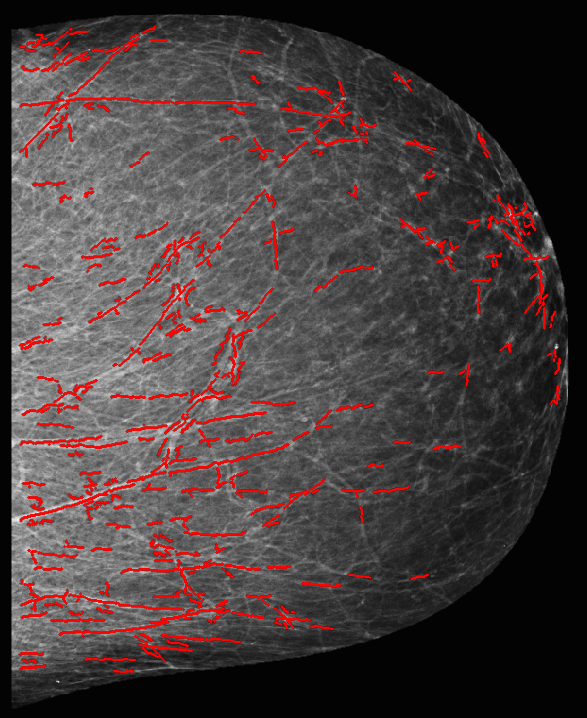
\includegraphics[width=0.5\textwidth]{Images/linear-structure.png}	
	\caption{Example image showing the orientated bins feature used to detect linear structure.}
\end{figure}

This operation results in two different filtered images. The first is the line strength image. Each pixel in the line strength image represents the average value from the maximum bin of the filtering. The second image represents the orientation and each pixel in the orientation image is a number representing the direction that the maximum bin was orientated in.

Once the line strength and orientation images have been generated the results can be enhanced by applying non-maximal suppression \cite{sonka2014image}. For each pixel in the line strength image non-maximal suppression selects the two pixels perpendicular to the current pixel based on the corresponding pixel in the line orientation image. If either of the two perpendicular neighbouring pixels are more intense than the current pixel the pixel is ignored. 

After suppression the image is once thresholded using a conservative value to remove noise and the image is converted to a binary image. A morphological dilation operation is used to improve the connectivity of the line shapes detected from the image by increasing the size very slightly to connect any disconnected components. Any points which are within an 8-connectivity of one another are counted as being part of the same structure.

The resulting shape features can be measured by standard first order statistics to produce descriptive features about the blobs and lines detected from the mammogram. As with blob features the detections were exported to a CSV file and then loaded into a IPython notebook for further analysis (as with blob features). Features created from the distribution of areas detected by the line features were:

\begin{itemize}
	\item Number of lines detected
	\item Average area
	\item Standard deviation of the areas
	\item Min \& max area
	\item 25/50/75 percentiles
	\item Count of areas above the mean.
\end{itemize}

\begin{figure}[H]
	\label{fig:feature-diagram}
	\centering
	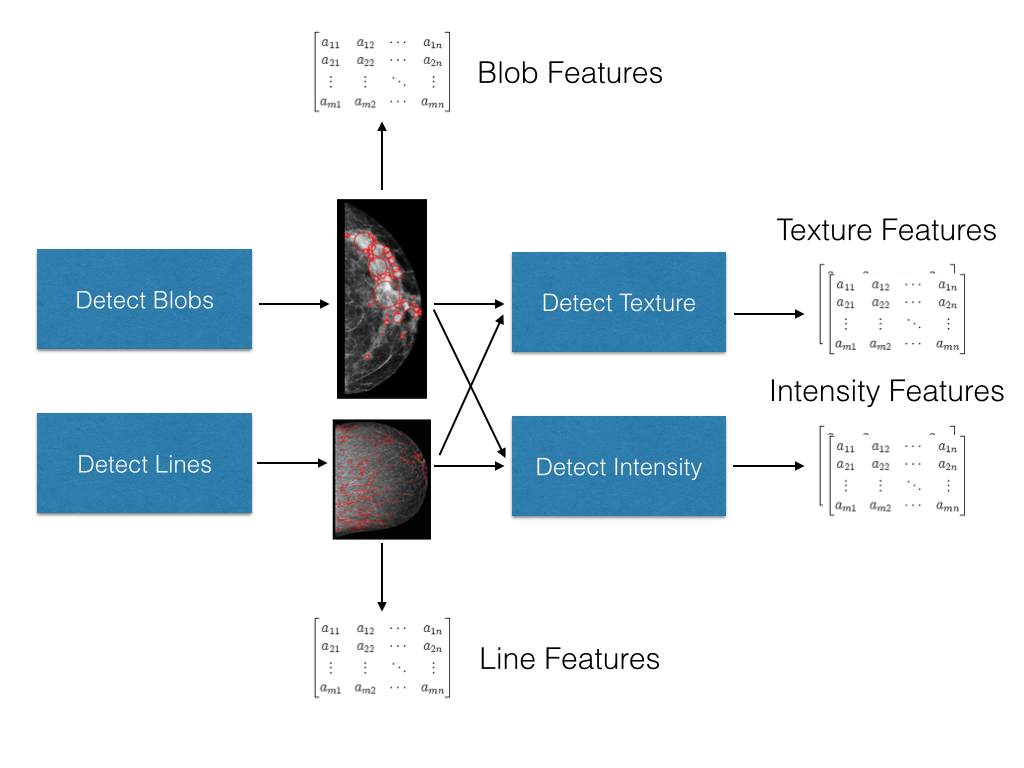
\includegraphics[width=0.9\textwidth]{Images/features-diagram.png}	
	\caption{Diagram showing how features are generated in the pipeline. First blobs and lines are detected and features are generated from these. These ROIs defined by these detections are then used to produce intensity and texture features.}
\end{figure}


\subsubsection{Intensity}
The shape features detected using orientated bins and multi-scale blobs define regions of interest across the breast. From these ROIs the patch of the image which is covered by the area or radius of the shape feature can be extracted. The histogram of the intensity values of this image patch provide can provide additional discriminative information about ROI. Descriptive statistics derived from the histogram of the ROI were computed. The final features derived were:

\begin{itemize}
	\item Number of intensity values
	\item Mean
	\item Standard deviation.
	\item Min \& max values
	\item 25/50/75 percentiles
	\item Skew
	\item Kurtosis
\end{itemize}

\subsubsection{Texture}
As with intensity features, texture features can be extracted from the patches defined by the shapes features as well. In this project we have only used texture features derived from the grey-level co-occurrence matrix \cite{haralick1973textural}. The properties computed from the co-occurrence matrices were homogeneity, dissimilarity, energy, and contrast. The definitions of each are given as the following:

Homogeneity:
\begin{equation}
	\sum\limits_{i,j=0}^{levels-1} \frac{P_{i,j}}{1+(i-j)^2}
\end{equation}

Dissimilarity:
\begin{equation}
	\sum\limits_{i,j=0}^{levels-1} P_{i,j}|i-j|
\end{equation}

Energy (or the square root of the angular second moment):
\begin{equation}
	\sqrt{ \sum\limits_{i,j=0}^{levels-1} P_{i,j}^2 }
\end{equation}

Contrast:
\begin{equation}
	\sum\limits_{i,j=0}^{levels-1} P_{i,j}(i-j)^2
\end{equation}

The experiments performed in chapter \ref{subsec:results-texture} all used a distance of 1 and a combination of eight different orientations of angles 0.0, 22.5, 45.0, 67.5, 90.0, 112.5, 135.0, 157.5 degrees.

When deriving texture and intensity features from ROIs defined by blobs features are generated for every blob detected. Because all of the detected blobs vary in scale, the final texture/intensity features are grouped and then averaged according to the scale of the ROI. In all experiments reported there were 10 scales. There were four texture features used so the resulting feature space was $4 \times 10 = 40$ dimensions. A similar process is used for intensity features derived from blobs. Lines are detected over only one scale so the results for each are simply averaged.

Some blob based texture/intensity features will produce zero entries for blobs of larger scales because there were none of that scale detected in that particular image. This causes the projections produced to be split into clusters according to what the size of the largest blob detected was. To prevent this unwanted effect zero entires were replace by the mean value for the relevant scale.

\subsection{Dimensionality Reduction}
In this project the three types of dimensionality reduction algorithm have been used to produce the lower dimensional representations from the higher dimensional feature spaces. The implementation of all algorithms used in this project are standard implementations available through the scikit-learn library.

Before running the dimensionality reduction algorithm the input feature matrix is standardised by removing the mean from each feature and scaling to standard variance. This ensures that the all of the features will roughly on the same scale as one another and therefore that the distance metric used to compute neighbours shouldn't be heavily weighted in favour of feature orders of magnitude larger than the others.

These three algorithms were chosen because they exhibit a variety of different properties. t-SNE is a fairly recent technique that is quite popular and is well known to produce good visualisations of higher dimensional data and is good at preserving local structure but fails to produce good global representations. Isomap was chosen in sharp contrast to this because it is a well know algorithm that attempts to preserve global structure but may not produce visualisations that are as good as t-SNE. LLE, being an approach based on eigendecomposition is similar to Isomap, but also preserve local structure over global structure similar to t-SNE. 

\subsection{Visualisation}
The visualisation aspects of this project have largely been handled by the inbuilt functionality that is available in the matplotlib and pandas Python libraries. However some additional visualisation techniques have also been implemented for and used for examining what the images look like for each point in the lower dimensional mapping.

\subsubsection{Visualisation of Images from Mapping}
In order to examine the how images change across the lower dimensional mapping and to try and understand why images are grouped closely together a small utility was created that would read in the mapping of the feature space and display a scatter plot of the mapping. When hovering over each point in the visualisation the image corresponding to that data point is displayed to the right of the scatter plot.


\begin{figure}[H]
	\label{fig:nd-viz}
	\centering
	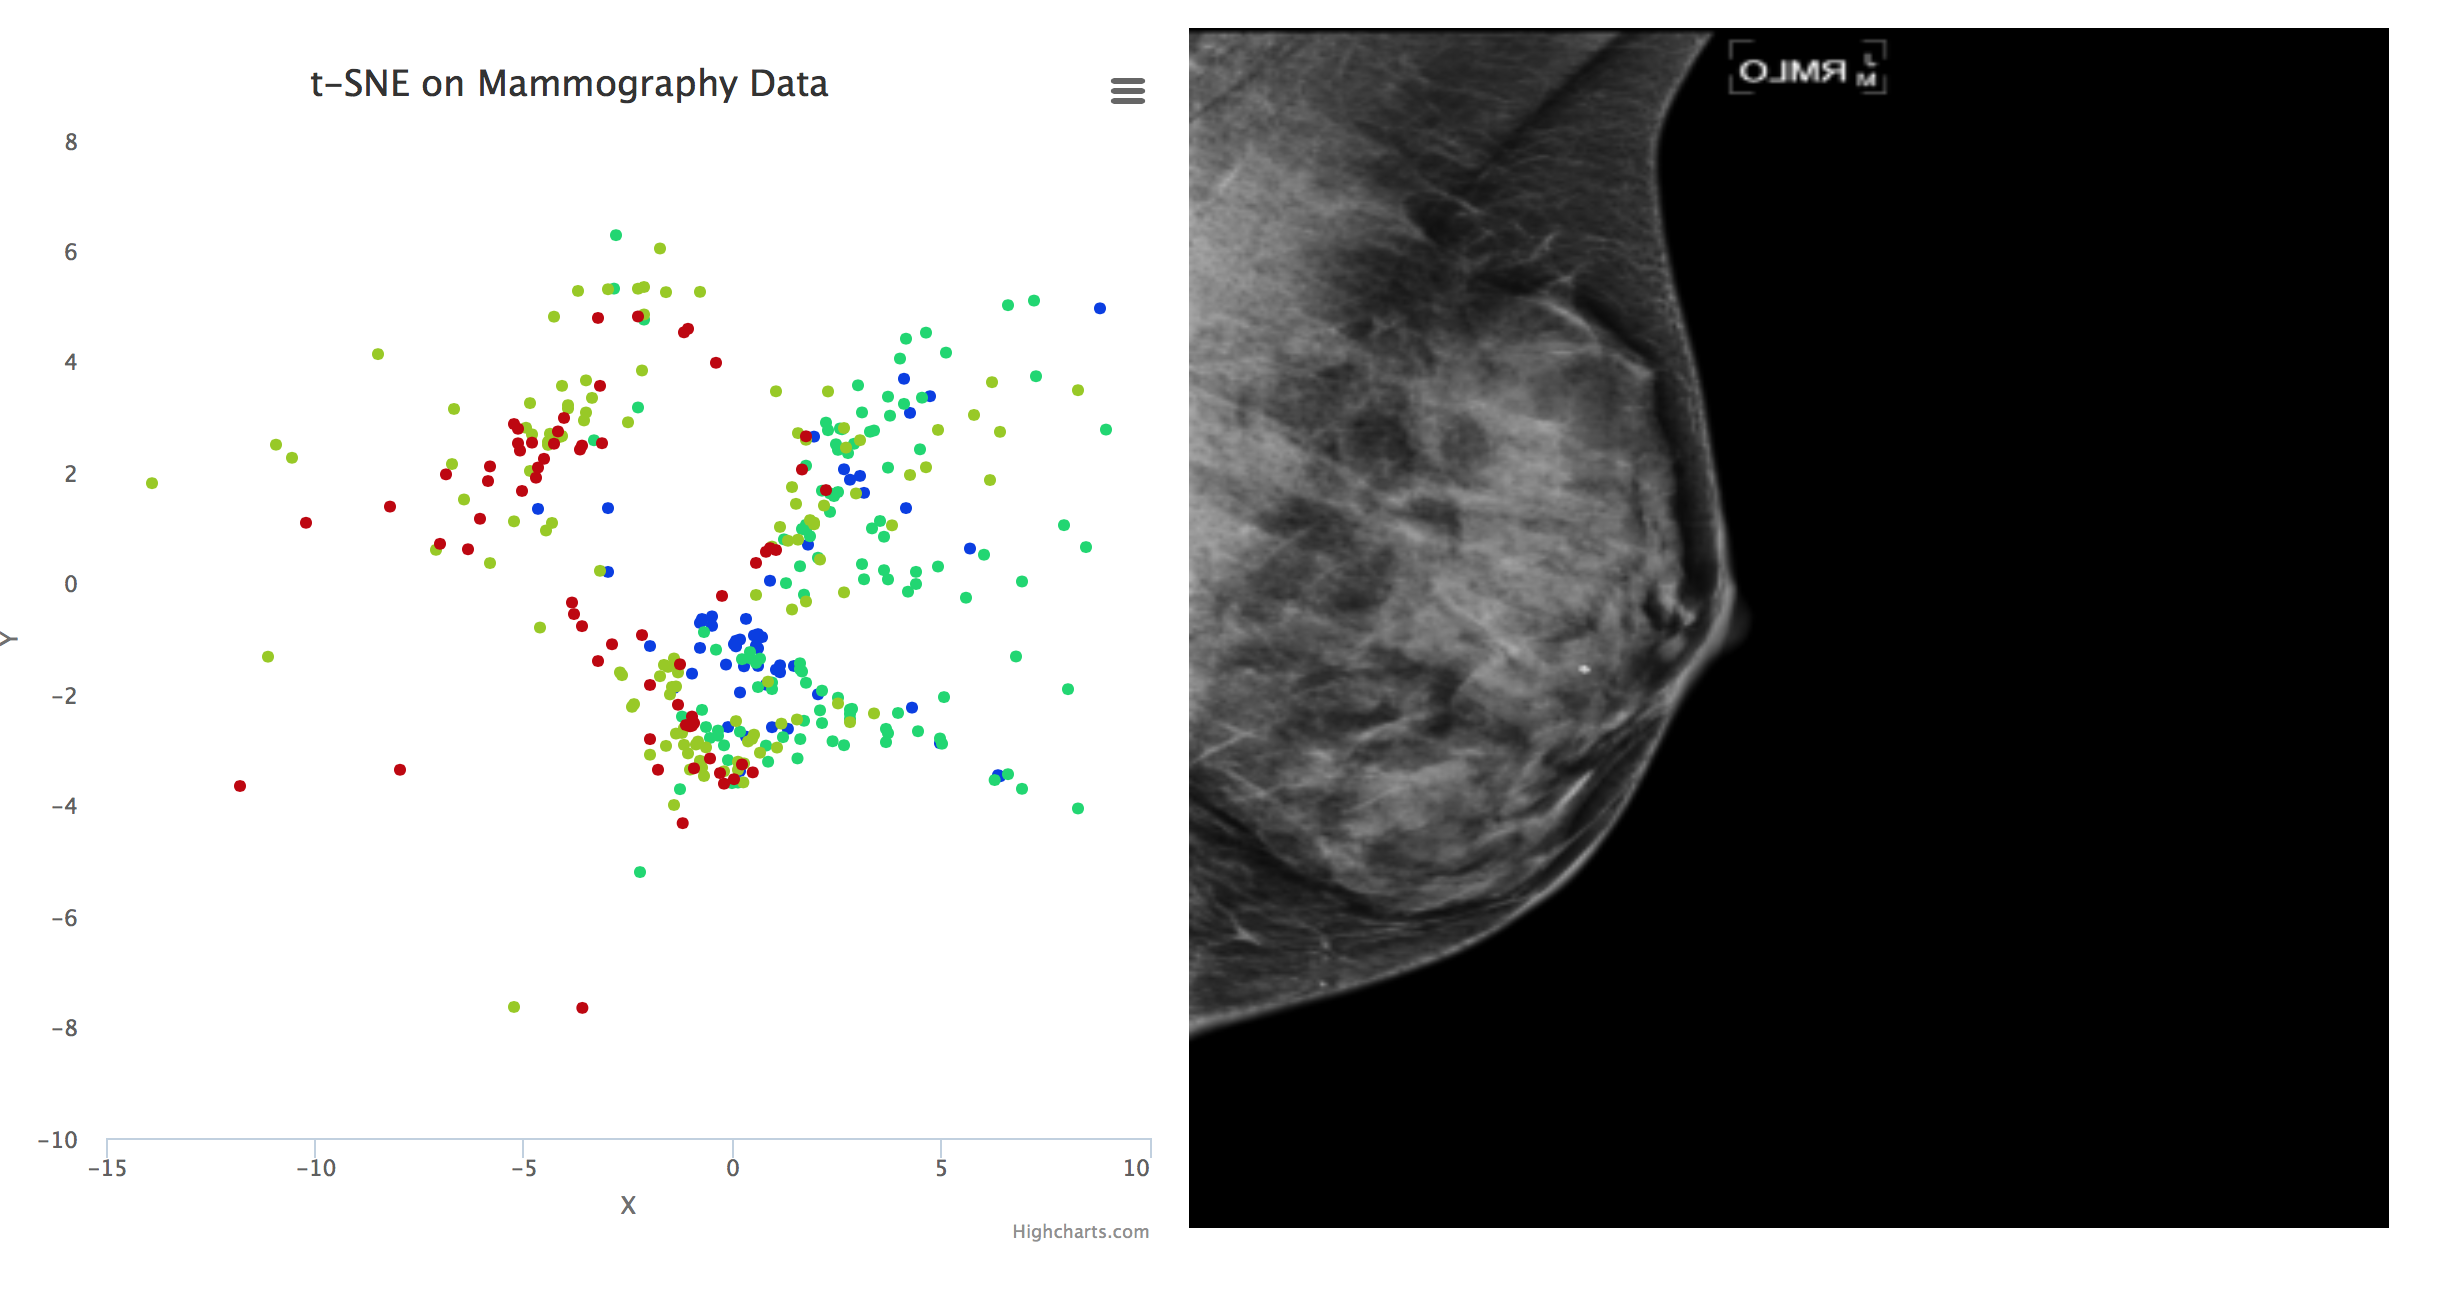
\includegraphics[width=0.9\textwidth]{Images/nd-viz.png}	
	\caption{Web based scatterplot visualisation tool. Hovering over points in the scatterplot on the left changes the image on the right to match the image corresponding to the data point.}
\end{figure}


This is the only part of the project that was not implemented in Python. Due to time constraints it was deemed not worth exerting a huge amount of time on developing this feature, but rather to just get something rapidly working. Ideally this would have been implemented in something like pyQt and utilised the matplotlib library. However, the actual implementation is written in JavaScript, HTML, and CSS. The main driving principle behind this is that it was quicker write some basic CSS to position the image and scatter plot next to one another than it was to write a proper Python GUI from scratch.

\subsubsection{Median Image Plot}

\begin{figure}[H]
	\label{fig:median-image}
	\centering
	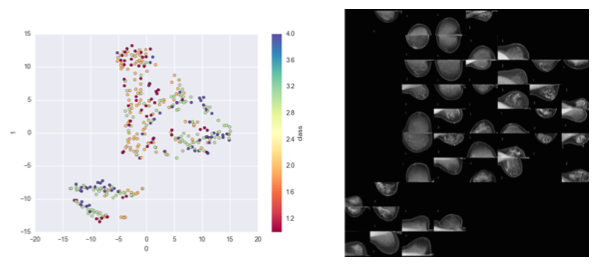
\includegraphics[width=0.8\textwidth]{Images/median-image.png}	
	\caption{The median image plotting routine takes a mapping and creates a 2D histogram. The ``median" image from each bin is then chosen to represent the whole bin.}
\end{figure}

Similarly to the previous visualisation this visualisation takes a projection of the feature space and creates a two dimensional histogram of the points. From each of the resulting bins the median point in both the $x$ and $y$ directions if found. The image which corresponds to this point is selected to be used as part of the visualisation. Each of the images is stitched together to form a matrix of images in the same shape as the lower dimensional mapping. Due to the huge size of mammographic images the images used in this visualisation are downscaled by a factor of 8. This keeps the visualisation generation performance reasonable at the expense of loosing some of the finer detail in the images.

\section{Datasets}
\label{sec:datasets}
Two different datasets were used as part of this project. One consisting of mammograms taken from a collection of real patients. The other dataset is a collection of artificially generated breast phantoms generously created by the University of Pennsylvania. 

\subsection{Real Data}
The dataset of real mammograms was taken from a private dataset captured using a Hologic full field digital mammography system. The dataset contains images of 90 unique patients each with a craniocaudal and mediolateral oblique view of both the left and right breasts, resulting in 360 total images. Each image in the dataset also has a corresponding binary breast mask. This mask is used to segment the  background and the pectoral muscle from the breast parenchyma.

\subsection{Synthetic Data}
The synthetic breast phantoms were generated by the University of Pennsylvania using the techniques outlined by Bakic et al. \cite{bakic2002mammogram1, bakic2002mammogram2, bakic2003mammogram3}. Their simulation system consists of three major components: a breast tissue model, a compression model, and an acquisition model. Adipose tissue compartments within the breast are modelled using thin shells in areas of primarily adipose tissue and as blobs in areas of predominantly fibroglandular tissue. Ductal lobes are also simulated by the model using a randomly generated tree. 

As the phantoms have not been formally assigned a BI-RADS class by an expert radiologist (as in the case of the real mammogram dataset) the ground truth for the risk associated with a particular mammogram is given by it's volumetric breast density (VBD). This information was supplied in the meta-data produced alongside the phantom mammograms.

None of the breast phantoms came with masks, but the masks are an essential part of blob detection. As none of the phantoms contain a pectoral muscle the masks were generated by simply using Otsu's method \cite{otsu1975threshold} to provide a threshold used to segment ``breast" from ``not breast" and create a binary mask for each phantom. 


\section{Comparison of Features}
\label{sec:comparison-of-features}
A comparison of the features can be made using the Kolmogorov-Smirnov two sample test. This is a non parametric test used to compare the difference between two probability distributions. In the one sample version of the test an empirical distribution function is compared with a reference cumulative distribution function (such as the normal distribution). The test quantifies the distance between the two distributions. The two sample version of the test is used to measure if two empirical distribution functions differ. Formally, the two sample Kolmogorov-Smirnov test is given by \cite{realStatsTwoSampleKStest}

\begin{equation}
	D_{m,n} = \max\limits_x | F(x) - G(x) |
\end{equation}

Where $F$ and $G$ are cumulative distribution functions of size $m$ and $n$ respectively. The null hypothesis that both samples come from a population that is similarly distributed can be rejected if $D_{m,n}$ is greater than the critical value for the corresponding significance level $D_{m,n,a}$ which is given by

\begin{equation}
	D_{m,n,a} = c(a) \sqrt{ \frac{m+n}{mn} }
\end{equation}

Where $c(a)$ is the inverse Kolmogorov distribution at $a$. The Kolmogorov-Smirnov two sample test can be applied to each feature extracted from both real and phantom mammograms. This will be used to quantitively compare how well each of the features extracted compare between datasets. 


\section{Evaluating the Quality of the Mapping}
As discussed in section \ref{sec:quality-measures} there are several quality metrics that can be used to measure the quality of a mapping produced from a dimensionality reduction algorithm which are independent of the technique being used.

In this project two different types of quality measures derived from the co-ranking matrix are implemented. The chosen metrics are trustworthiness and continuity and the local continuity meta-criteria. These metrics were chosen because together they can be used to measure both the false positives/negatives present in the mapping (for trustworthiness and continuity) and the true positives/negatives (LCMC). 

\section{Implementation}
\label{sec:implementation}
This section provides a brief overview of the implementation details used in the project. All of the methods discussed in the preceding sections were implemented in Python. The technical output of the project is a Python library and command line tool which is used to create the methods discussed in the first part of this chapter.

The final implementation produced for this project is a Python library that includes a small command line interface. The feature detection part of the pipeline takes a long time to process and subsequently the commands for running this were made into a CLI that can be left to run overnight. 

However the second half of the ``pipeline" has not been fixed in the same way. The subsequent analysis of the generated features was performed by means of a IPython notebooks. This was not made into a fixed pipeline because it is often desirable to explore the extracted features in an interactive way. Instead commonly performed operations were identified and moved the most appropriate module as the project progressed. This evolved over time into the final submitted API. 

\subsection{Python Package}
The majority of the components used in the project are built upon the top of the scipy stack \cite{jones2014scipy}. Two major additional libraries (which also rely on the scipy stack) which have been used heavily in the project are the scikit image \cite{van2014scikit} and scikit learn \cite{pedregosa2011scikit} projects.

The library created as part of this project forms a complete python package. The package consists of five top level modules and a collection of submodules implementing specific functionality relating to the features detected by the system. The description of each of the modules is as follows:

\begin{itemize}
	\item {\bf analysis}: The analysis module implements commonly used functions used to analyse the images after feature extraction has been performed. These functions are typically called directly from the python interpreter to in a IPython notebook session.
	\item {\bf coranking} This module contains the code for computing the co-ranking matrix form two representations of the same dataset.
	\item {\bf plotting}: This module provides a collection of custom, convenience plotting functions that largely depend on the matplotlib library.
	\item {\bf io\_tools}: The io\_tools module implements functions for iterating over directories of images and there corresponding masks as well as image loadings and preprocessing functions.
	\item {\bf utils}: The utils module contains a collection of miscellaneous helper functions used in various places throughout the package.
\end{itemize}

In order to automatically detect features across a whole dataset of images a sub-package called reduction was created. This package handles the loading and multiprocessing of multiple images in a dataset. While most of the implementation of done as a purely functional API sub-package was developed using classes to make it more easily extensible for new image reductions.

\begin{itemize}
	\item {\bf reduction}: Contains an abstract class Reduction which defines a generic reducer interface. This is a super class to all processes that require iterating over a dataset to carry out an operation on each image (i.e. feature detection).
	\item {\bf multi\_processed\_reduction}: Derived from the Reducer class in the reduction module this adds multiprocessing support to the original reducer base class. (see subsection \ref{subsec:multiprocessing}
	\item {\bf reducers}: This is a collection of classes that implement the Reduction and MultiProcessedReduction abstract classes to provide specific functionality for each feature detection process.
\end{itemize}

An additional sub-package contains the modules used by the reduction sub-package to perform feature extraction. The package includes the following modules:

\begin{itemize}
	\item {\bf blobs}: Contains the code implementing blob detection using the approach outlined in section \ref{sec:features}. This also uses an additional private module which provides the code for the graph built as part of the blob merging scheme.
	\item {\bf linear\_structure}: Contains the code implementing line feature detection using the approach outlined in section \ref{sec:features}. This also uses a couple of additional private modules within the sub-package which provide the code for non-maximal suppression and the orientated bins feature. 
	\item {\bf texture}: Contains the code for computing the GLCM and texture features from ROIs.
	\item {\bf intensity}: Contains the code for computing first order statistics from ROIs.
\end{itemize}

The last part of the library is the deformable convolution module. This implements the deformable convolution approach outlined by Chen et al \cite{chen2013multiscale}. Due to the performance considerations associated with convolution I chose not to write this module directly in Python but to implement it as a C function which is compiled directly using the Python C API.

\subsection{Command Line Interface}
The command line tools offered by the program are built using the Click library \cite{clickLibrary}. The CLI provides a thin wrapper to the some of the higher level library functions available in the package. The most important commands offered by the CLI are those concerned with image processing to collect features from the images. These functions involve iterating over a folder of images and applying the feature extraction techniques outlined in section  \ref{sec:features}. These operations can take in the order of several hours to complete and so it is useful to have them exposed on the command so they can be run and left until complete. 

These commands for image reduction also add the ability to automatically dump the output of the reduction to a CSV file named by the user upon completion. Typically these commands take two directories (one for the images and one for the masks) and the name of the output file. In the case of intensity and texture features they also take an additional file containing the ROIs from which to extract features.

\subsection{Multiprocessing}
\label{subsec:multiprocessing}
The image processing component of the pipeline created for this project is extremely time consuming. The two shape features used in this project take up to a minute to process a single image. The biggest contribution to the running time is the filtering and convolution of the images. Sadly this is an operation that is intrinsically complex and therefore slow. However, since the processing of an image is completely separate from all other images multiprocessing support becomes an option. 

The feature detection routines produces as part of the Python package all support multiprocessing through the Python multiprocessing module. Each routine has support to use an unlimited number of threads although in practice the physical limitations of the computer hardware used limited the number to just two. Despite only using one additional process this still managed to speed up the feature detection routines for the whole set of images by several hours.



